\chapter{CẤU TẠO NGUYÊN TỬ}
\section{Thành phần nguyên tử}
\subsection{NỘI DUNG BÀI HỌC}
\subsubsection{SỰ PHÁT TRIỂN MÔ HÌNH NGUYÊN TỬ}
\begin{hoplythuyet}
	\begin{minipage}[htp!]{0.5\textwidth}
		Từ thời cổ Hy Lạp,nhà triết học Democritous (Đê-mô-crít) (Hình \ref{fig:Democritus})
		Mọi thứ trên thế giới đều được tạo ra từ các hạt nhỏ không thể chia nhỏ được nữa được gọi là \textbf{“nguyên tử”}, có nghĩa là \textbf{“không thể thay đổi được”}
	\end{minipage}
	\begin{minipage}[htp!]{0.5\textwidth}
		\begin{center}
			
\includegraphics[width=3cm]{DEMOCRITUS}
			\captionof{figure}{Democritus (460 - 370,Hy Lạp)\label{fig:Democritus} }
		\end{center}
	\end{minipage}
	
	\begin{center}
		\includegraphics[width=12cm]{Historyatom}
		\captionof{figure}{Lịch sử phát triển mô hình nguyên tử \label{fig:Historyatom} }
	\end{center}
\end{hoplythuyet}
\subsubsection{Thành phần và cấu trúc của nguyên tử}
\paragraph{Thành phần}
\begin{hoplythuyet}
	Nguyên tử gồm hạt nhân chứa proton, neutron và vỏ nguyên tử chứa electron.
	\begin{center}
		\includegraphics[width=9cm]{mohinhnguyentu}
		\captionof{figure}{Mô hình nguyên tử}
	\end{center}
\end{hoplythuyet}
\paragraph{Sự tìm ra electron}
\ntd{Thí nghiệm khám phá tia âm cực của Thomson}\\
Năm 1897, J. J. Thomson (Tôm-xơn, người Anh) thực hiện thí nghiệm phóng điện qua không khí loãng đã phát hiện ra chùm tia phát ra từ cực âm.(xem hình \ref{fig:hinh3} ) và link video bằng mã QR ở bên dưới.\\ 
\hinhphai{\begin{center}
		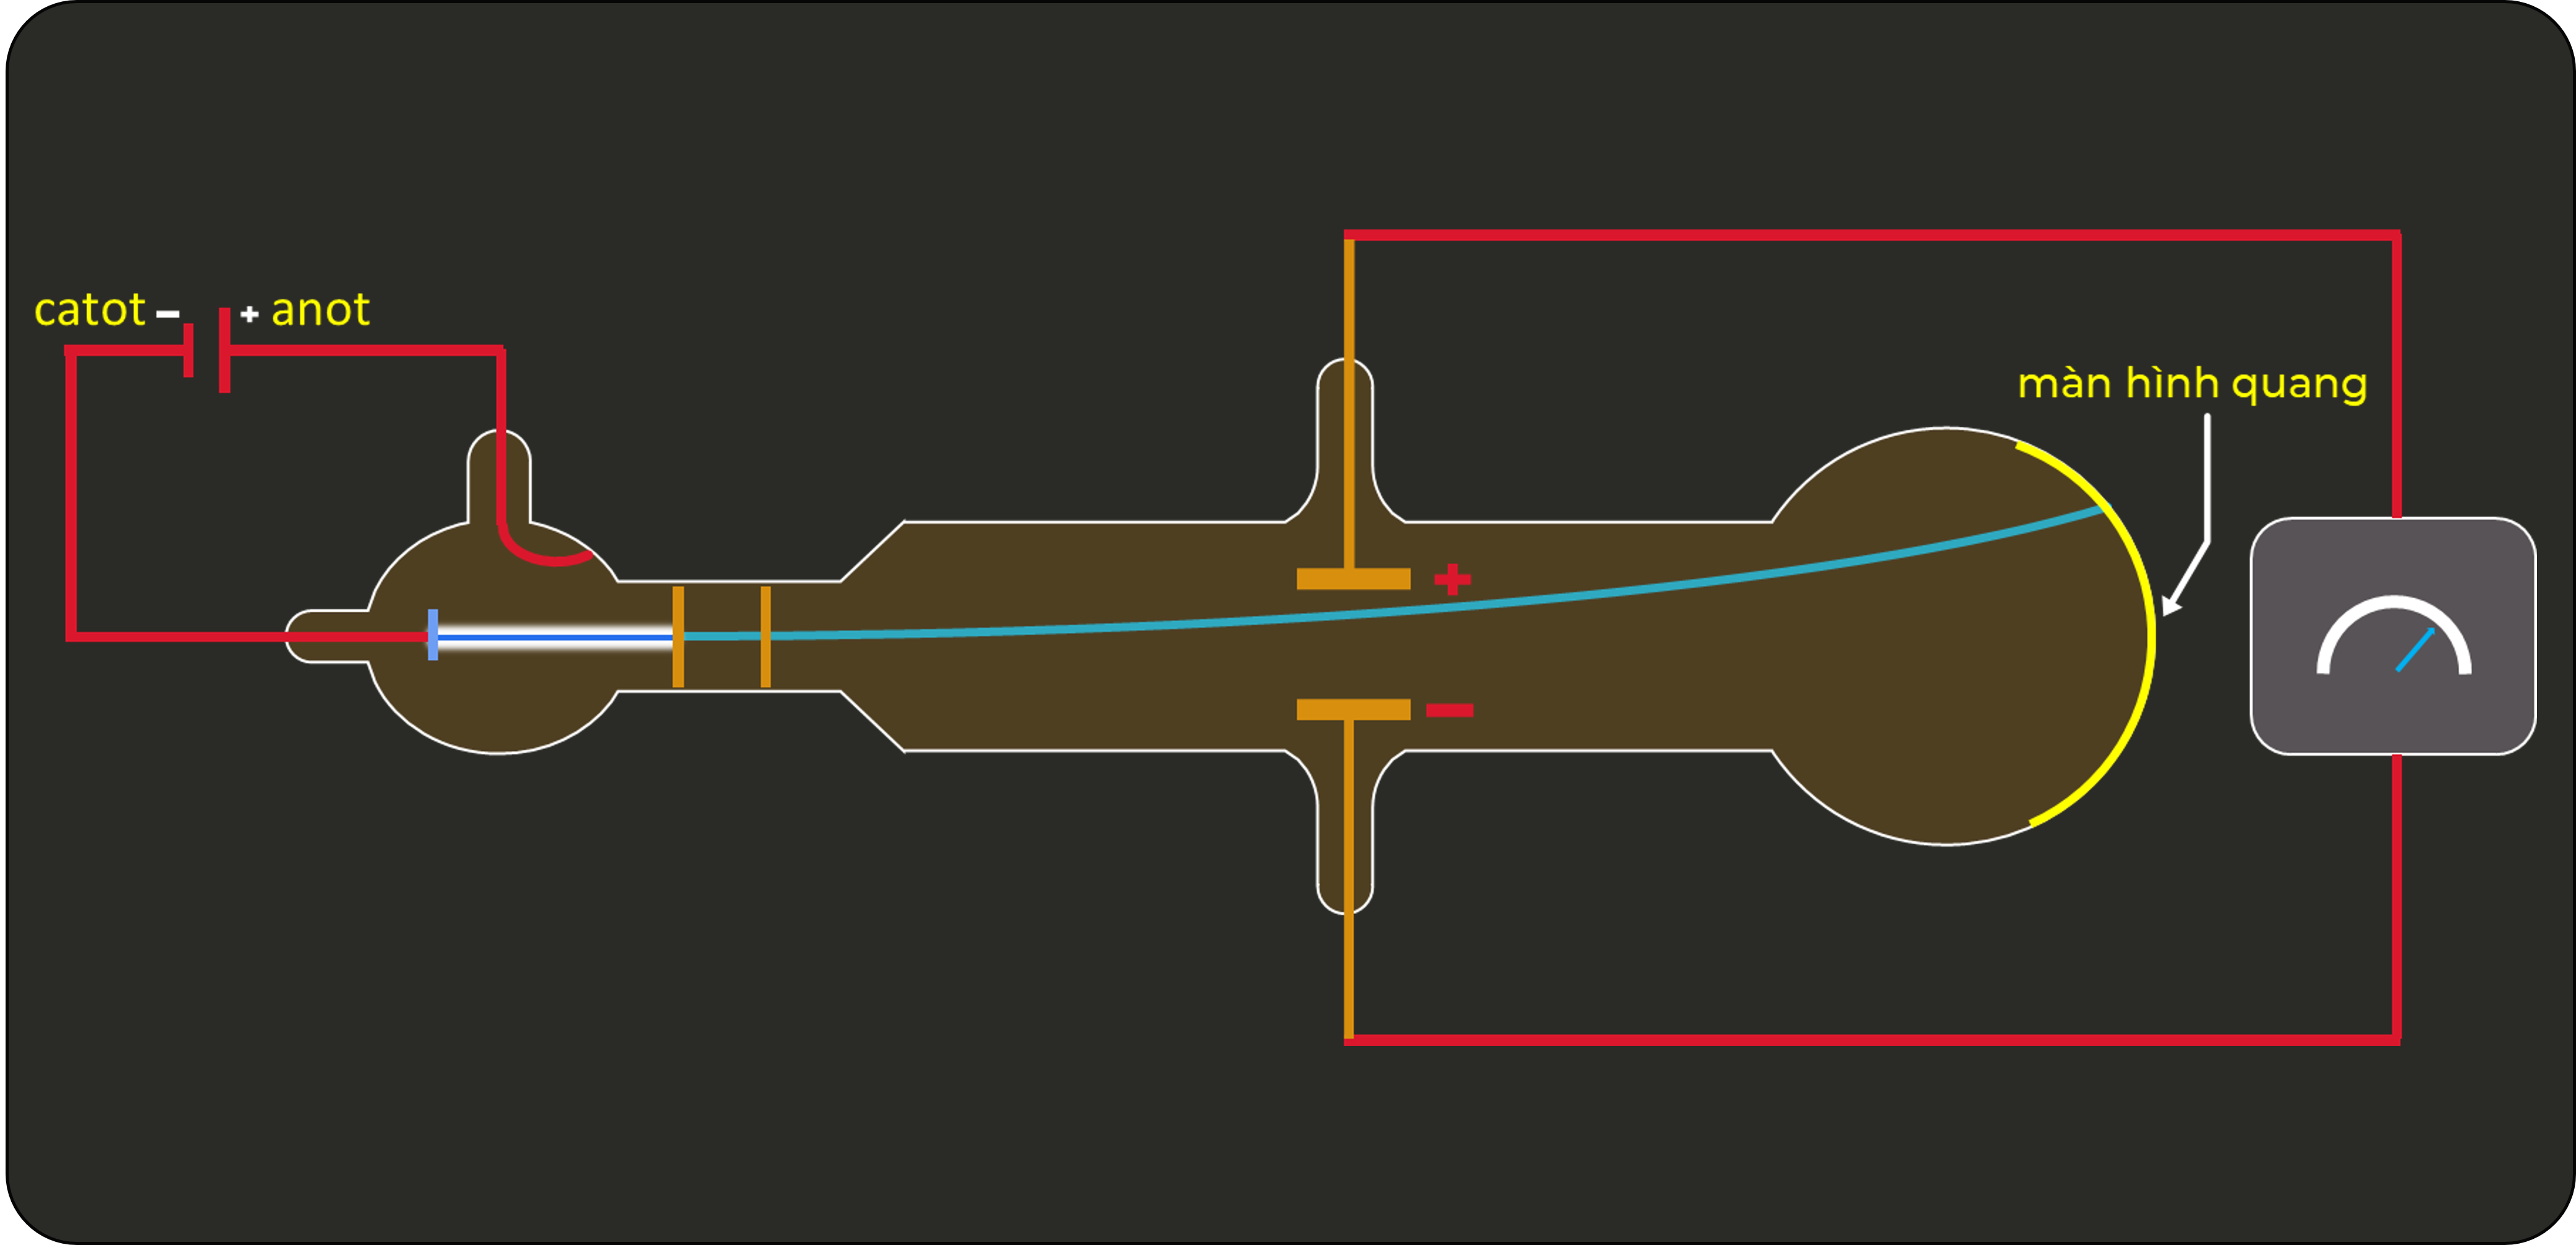
\includegraphics[width=9cm]{TNTHOMSON}\\
		\captionof{figure}{Thí nghiệm của Thomson}
		\label{fig:hinh3}
\end{center}}{\begin{tikzpicture}
		\path (0,0)  node (QRCODE) {\qrcode[height=2.0cm]{https://youtu.be/y2uswXtC5O8}}
		(QRCODE.south) node[anchor=north]{(\fmmfamily Các bạn  dùng ~\rotatebox{-15}{\faMobile}~quét mã QR để xem video TN nhé!)}
		;
\end{tikzpicture}}






\begin{hoivadap}
	Vai trò của lớp bột huỳnh quang trong thí nghiệm ở hình \ref{fig:hinh3}
	\huongdan{\taodongke{10}}
\end{hoivadap}

\begin{hoivadap}
	Quan sát Hình \ref{fig:hinh3} và video , giải thích vì sao tia âm cực bị hút về cực dương của trường điện.
	\huongdan{\taodongke{10}}
\end{hoivadap}

\begin{hoivadap}
	Nếu đặt một chong chóng nhẹ trên đường đi của tia âm cực thì chong chóng sẽ quay. Từ hiện tượng đó, hãy nêu kết luận về tính chất của tia âm cực.
	\huongdan{\taodongke{5}}
\end{hoivadap}
\newpage
\vspace*{6pt}
\begin{emcobiet}
	Mô hình Thomson còn gọi là mô hình \lq\lq bánh pudding mận".Theo Thomson:
	\begin{enumerate}
		\item Nguyên tử là quả cầu mang điện tích dương, bên trong chứa các êlectron.
		\item Nguyên tử trung hòa về điện.
	\end{enumerate}
	
\end{emcobiet}


\paragraph{Sự khám phá hạt nhân nguyên tử}
\ntd{Tìm hiểu thí nghiệm của Rutherford}\\
Năm 1911, E. Rutherford (Ro-dơ-pho, người Niu Di-lân) thực hiện thí nghiệm bắn phá lá vàng rất mỏng bằng chùm hạt $ \alpha $ \footnote{Hạt $\alpha$ : hạt nhân helium, mang điện tích dương.} (xem hình \ref{fig:hinh4})
\begin{center}
	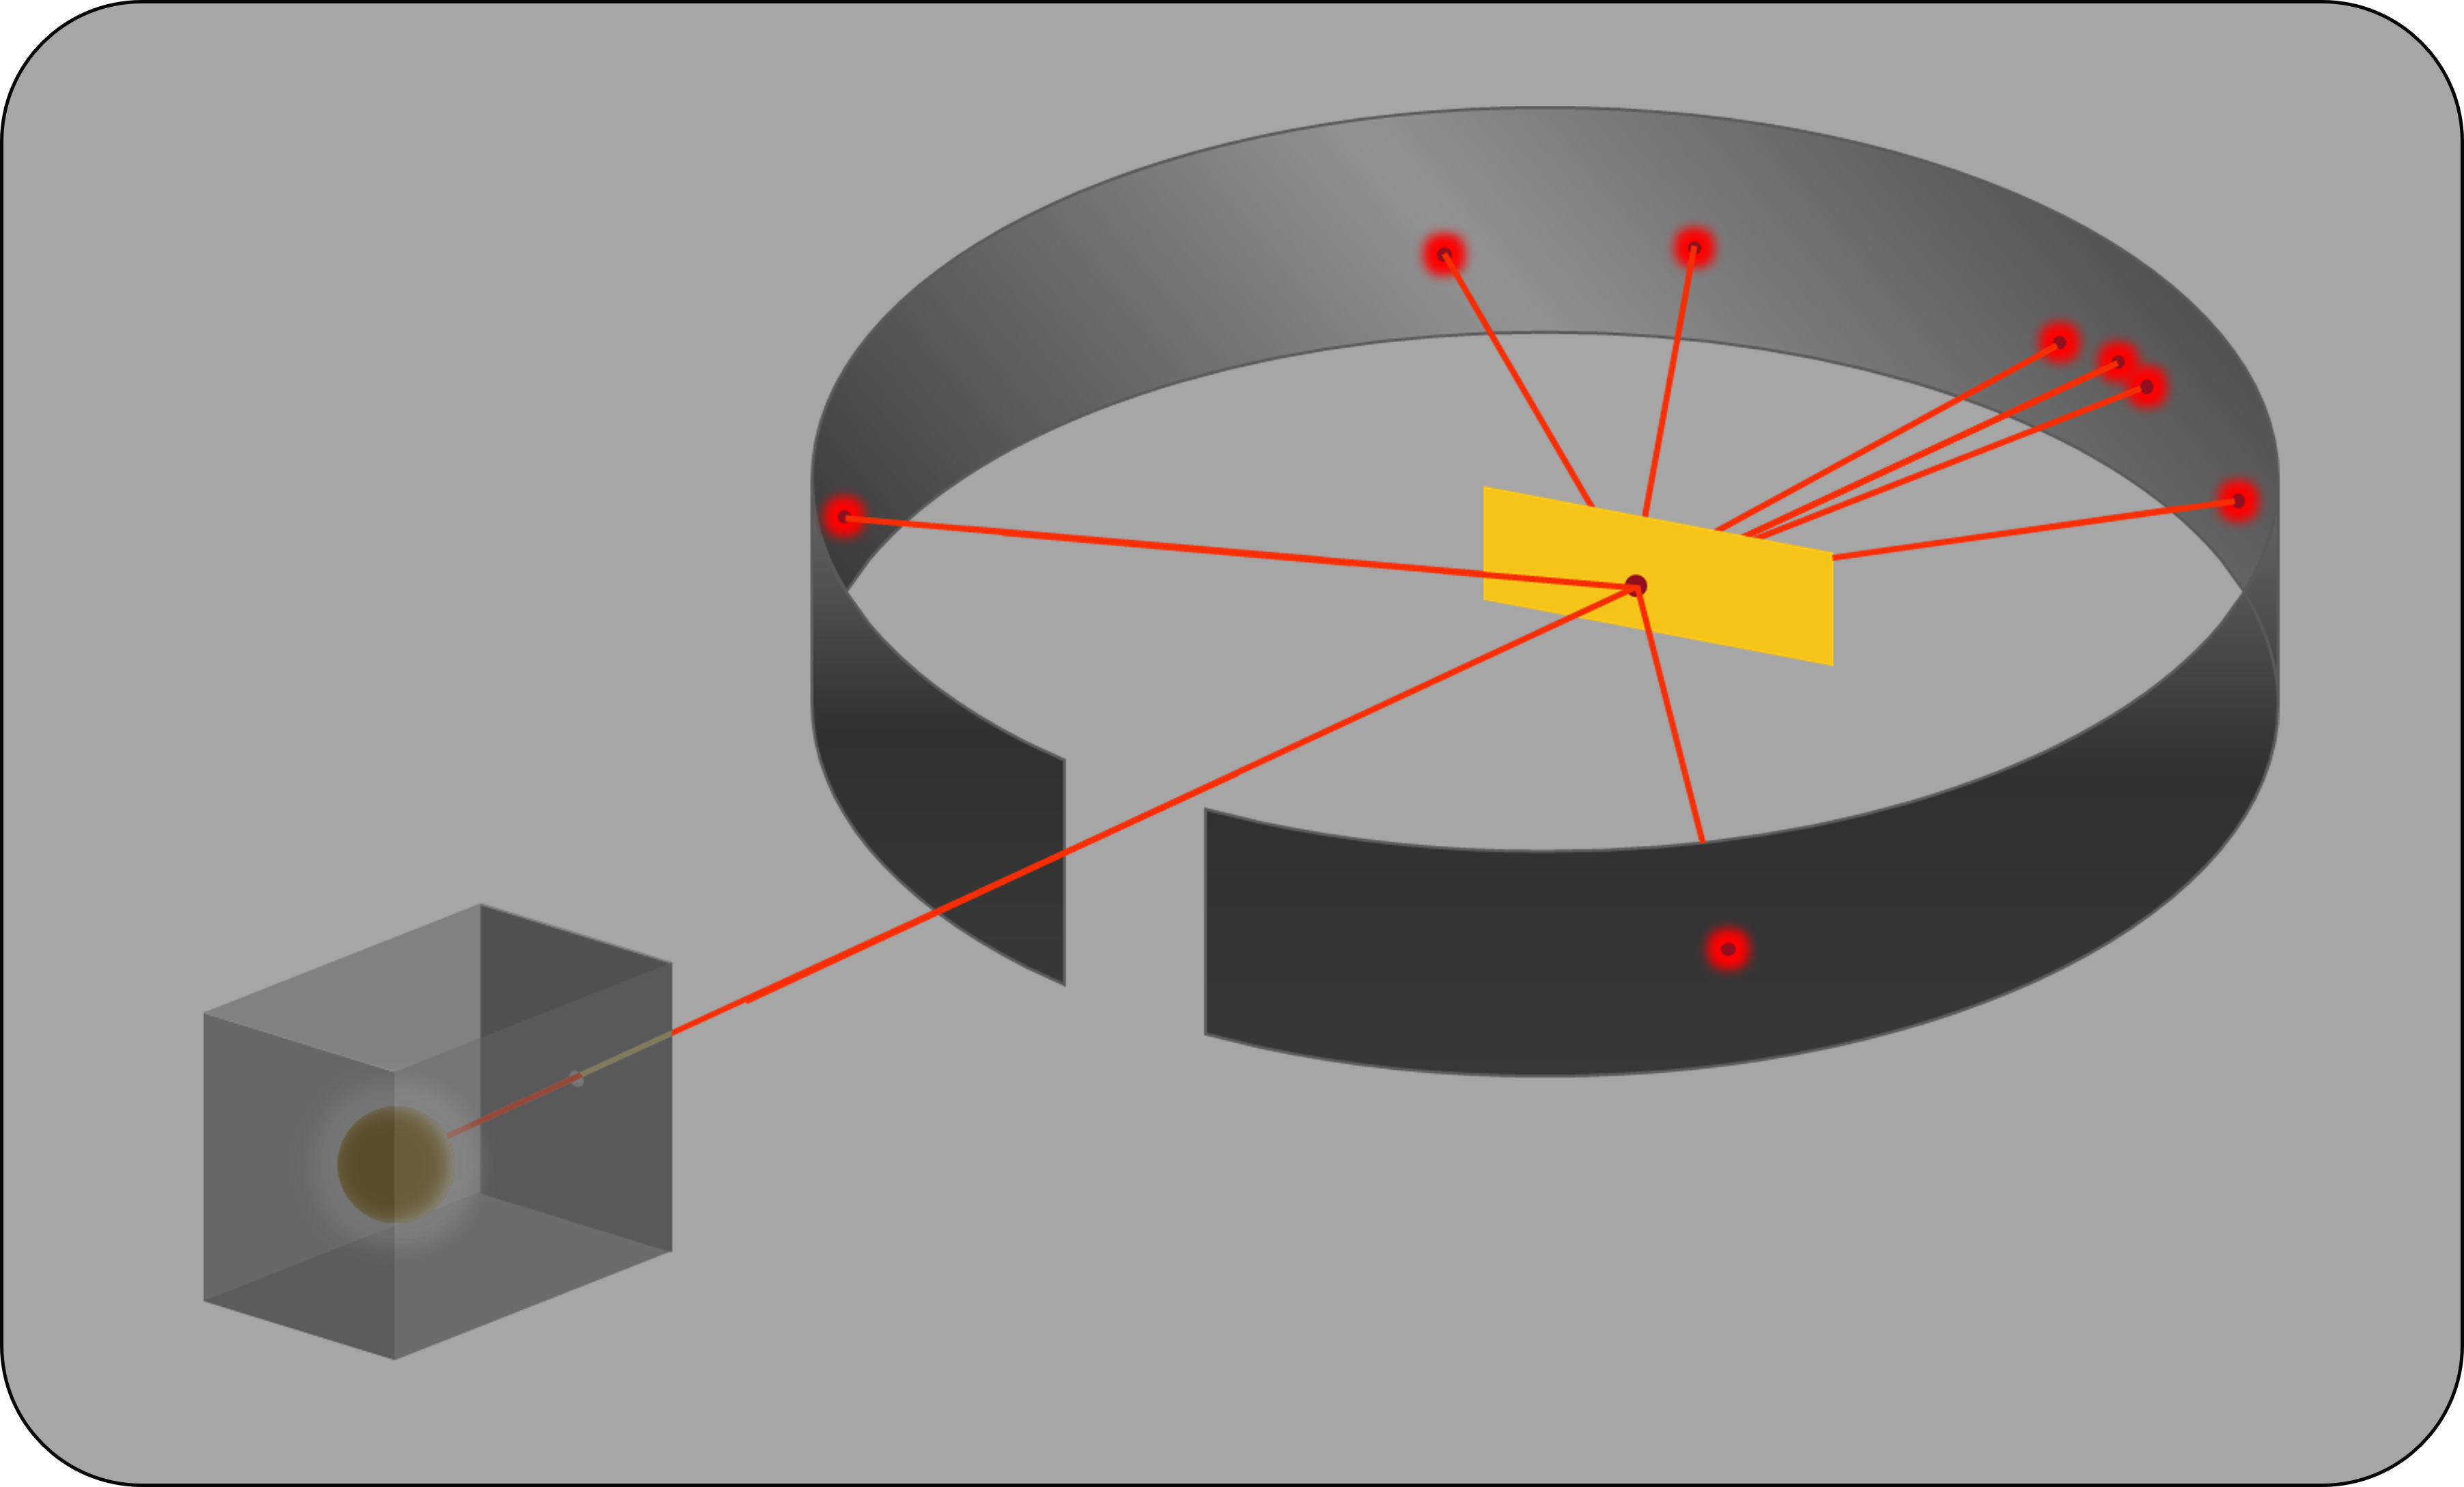
\includegraphics[width=9cm]{TNRUTHERFORT}\\
	\captionof{figure}{Thí nghiệm của Rutherford}
	\label{fig:hinh4}
\end{center}

\begin{center}
	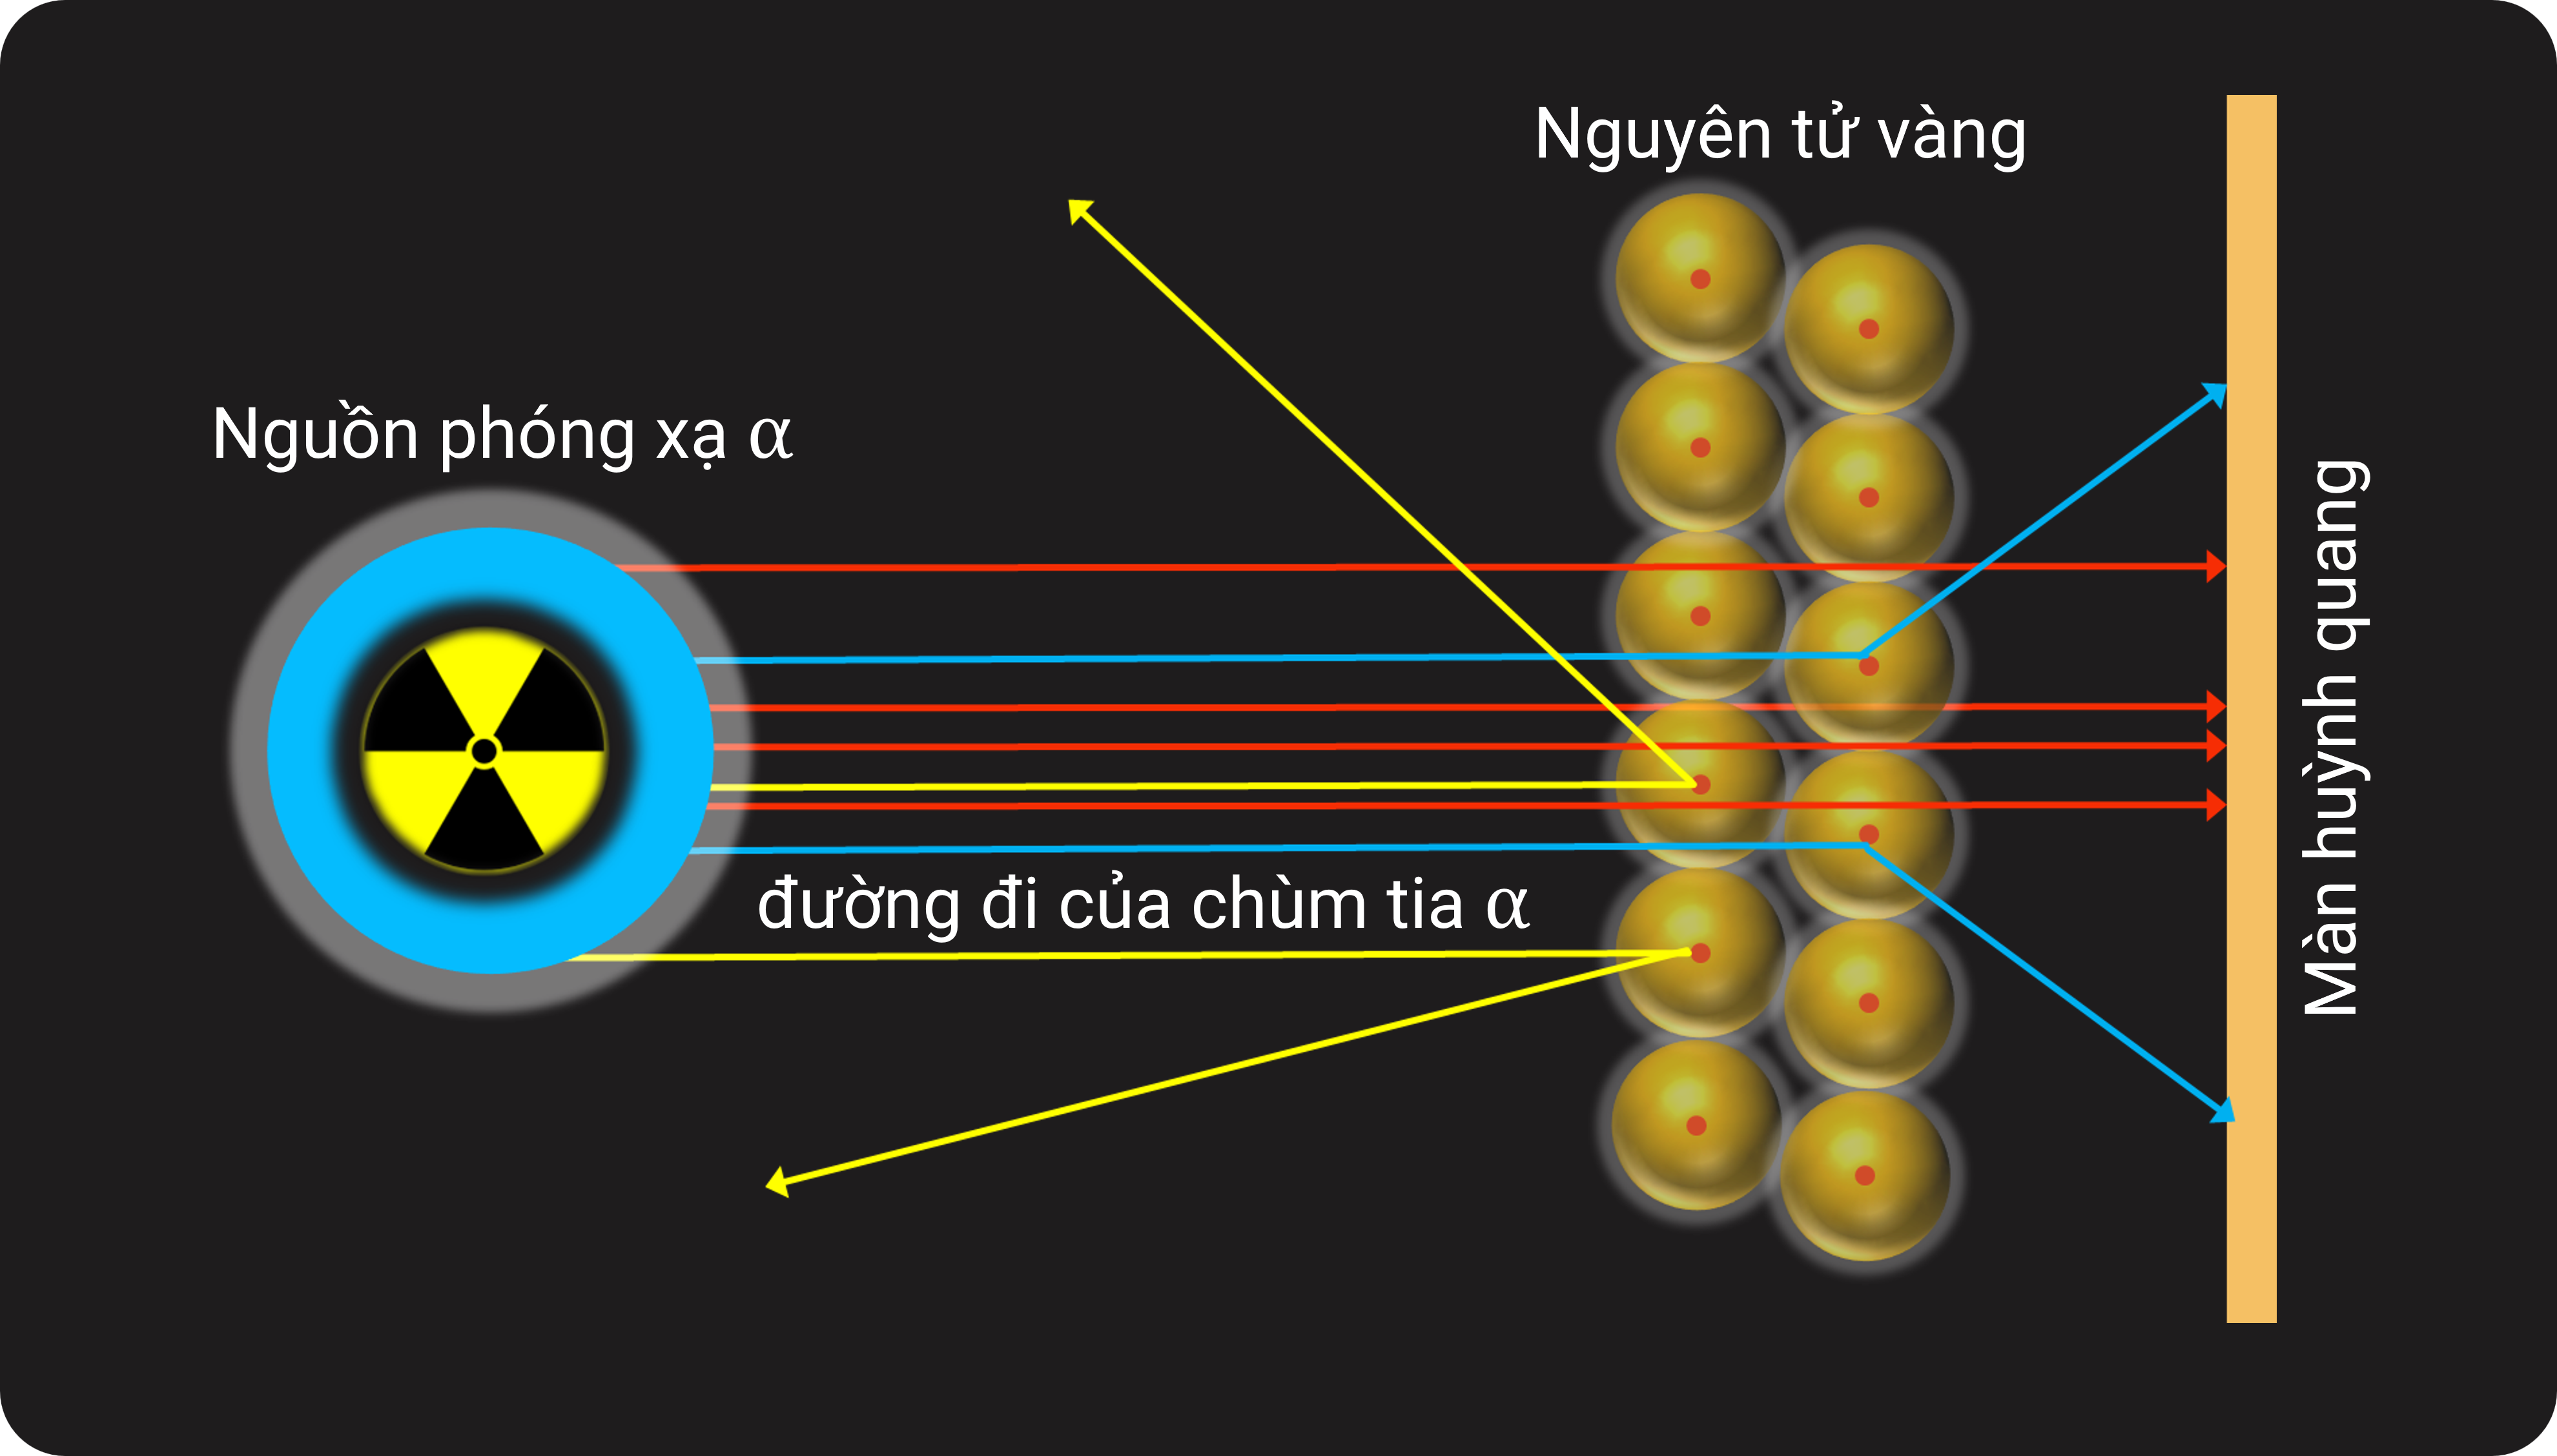
\includegraphics[width=9cm]{KQTN}\\
	\captionof{figure}{Kết quả thí nghiệm của Rutherford}
	\label{fig:hinh5}
\end{center}

\begin{hoivadap}
	Quan sát hình \ref{fig:hinh4}, cho biết các hạt $\alpha$ có đường đi như thế nào. Dựa vào Hình \ref{fig:hinh5} , giải thich kết quả thí nghiệm thu được.
	\huongdan{\taodongke{5}}
\end{hoivadap}
\vspace*{6pt}
\begin{hoplythuyet}
	{\bfseries{Kết luận}}
	\begin{itemize}
		\item Nguyên tử có cấu tạo rỗng, gồm hạt nhân ở trung tâm và lớp vỏ là các electron chuyển động xung quanh hạt nhân.
		\item Nguyên tử trung hoà về điện: số đơn vị điện tích dương của hạt nhân bằng số đơn vị điện tích âm của các electron trong nguyên tử.
	\end{itemize}
\end{hoplythuyet}
\paragraph{Cấu tạo hạt nhân nguyên tử}
\begin{center}
	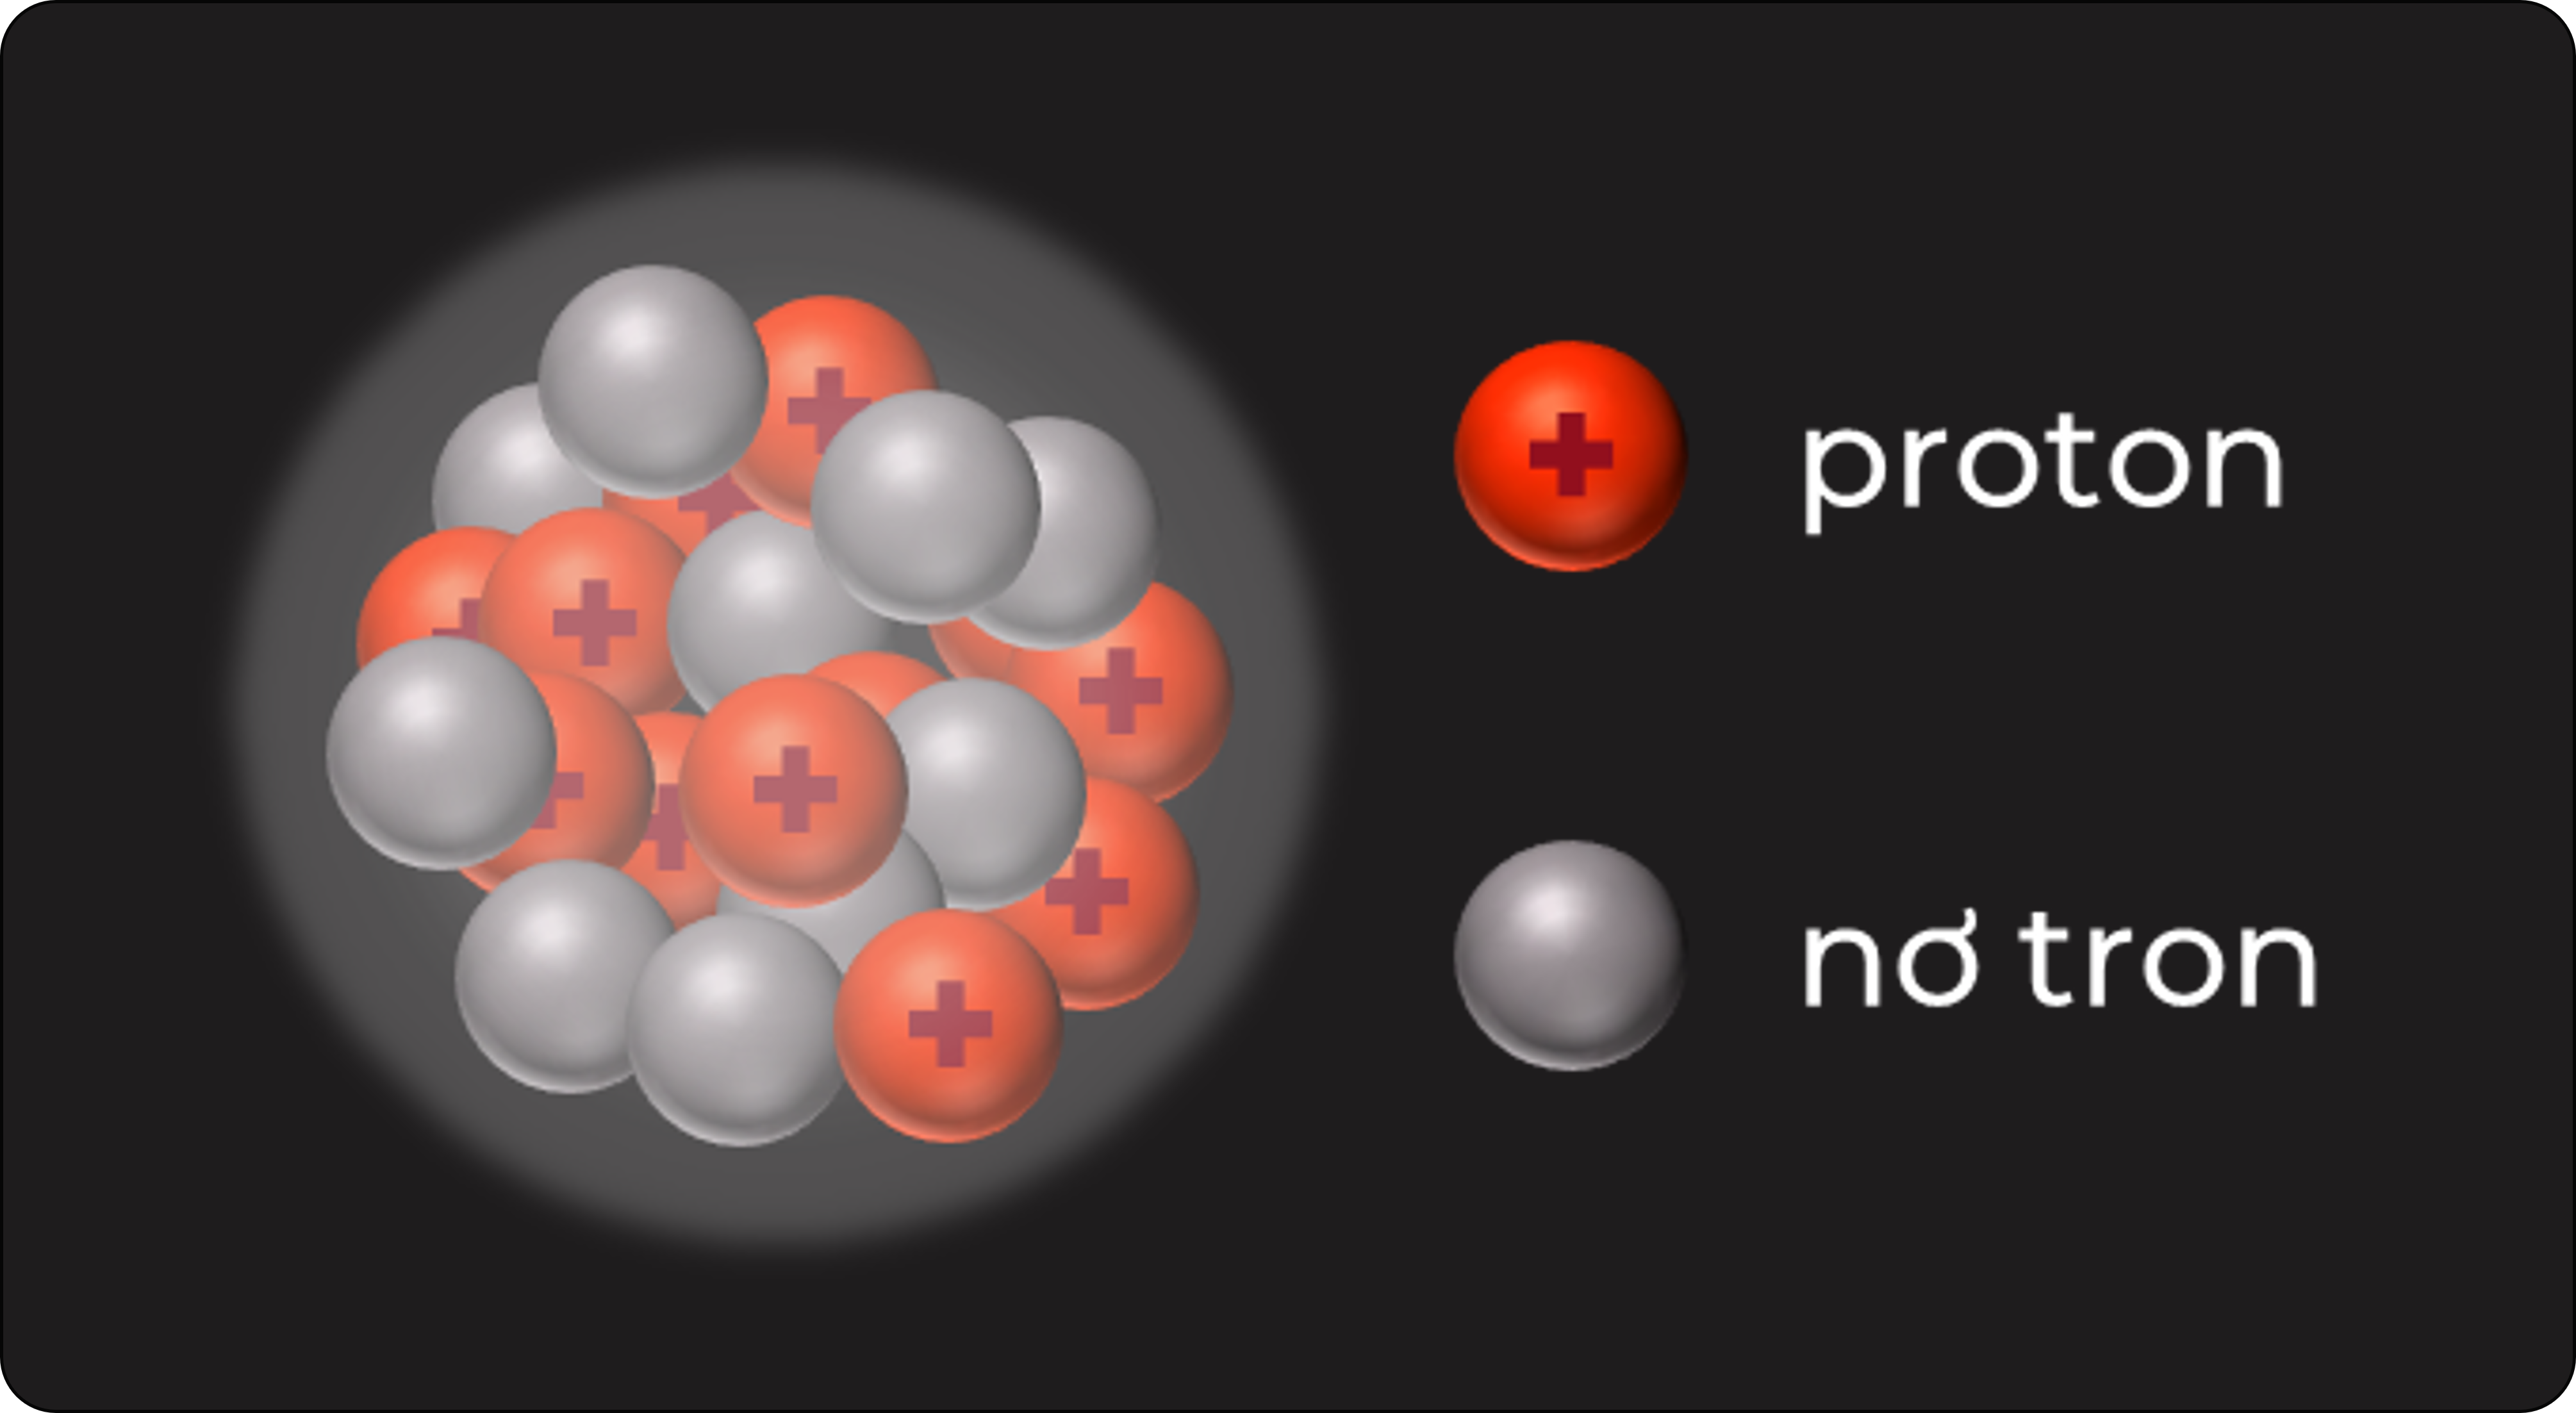
\includegraphics[width=9cm]{CAUTAOHATNHAN}\\
	\captionof{figure}{Thành phần của hạt nhân}
	\label{fig:hinh6}
\end{center}
\begin{hoivadap}
	Quan sát hình \ref{fig:hinh6} và kết hợp SGK , các bạn hãy nêu thành phần của hạt nhân
\end{hoivadap}
\begin{hoplythuyet}
	Proton, neutron và electron là các hạt cấu tạo nên nguyên tử.
\end{hoplythuyet}
\begin{tongket}
	Thành phần cấu tạo của nguyên tử gồm:
	\begin{itemize}
		\item  Hạt nhân (nucleus): ở tâm của nguyên tử, chứa các proton mang điện tích dương và các neutron không mang điện.
		\item Vỏ nguyên tử: chứa các electron mang điện tích âm, chuyển động rất nhanh xung quanh hạt nhân.
		\item Trong nguyên tử, số proton bằng số electron nên nguyên tử trung hoà điện.
		\item Khối lượng của electron rất nhỏ, không đáng kể so với khối lượng của proton hay neutron nên khối lượng của nguyên tử tập trung hầu hết ở hạt nhân.
	\end{itemize}
\end{tongket}


\begin{longtable}{|c|c|c|c|c|c|}
	\caption{\indam[dndo]{Khối lượng, điện tích của các loại hạt cấu tạo nên nguyên tử}}
	\label{tab:table1}\\
	\hline
	\rowcolor{dnxanh!25} \indam[dnxanh]{Hạt} & \indam[dnxanh]{Kí hiệu} & $\begin{array}{c}\text {\indam[dnxanh]{Khối lượng} } \\
		\text {\indam[dnxanh]{(kg)}  }\end{array}$ & \indam[dnxanh]{Khối lượng (amu)} & $\begin{array}{c}\text { \indam[dnxanh]{Điện tích} } \\
		\text { \indam[dnxanh]{(C)} }\end{array}$ & $\begin{array}{l}\text { \indam[dnxanh]{Điện tích} } \\
		\text { \indam[dnxanh]{tương đối} }\end{array}$ \\
	\hline\endhead
	\rowcolor{dnvang!15} Proton & $p$ & $1,672 \cdot 10^{-27}$ & $\approx 1$ & $1,602 \cdot 10^{-19}$ & +1 \\
	\hline
	\rowcolor{dnvang!15} Neutron & $\mathrm{n}$ & $1,675 \cdot 10^{-27}$ & $\approx 1$ & 0 & 0 \\
	\hline\rowcolor{dnvang!15} Electron & e & $9,109 \cdot 10^{-31}$ & $\begin{array}{c}
		~ \\
		\dfrac{1}{1837} \approx 0,00055\\
		~ \\
	\end{array}$ & $-1,602 \cdot 10^{-19}$ & -1 \\
	\hline
\end{longtable}
\paragraph{KíCH THƯỚC VÀ KHỐI LƯợNG NGUYÊN TỬ}
\begin{center}
	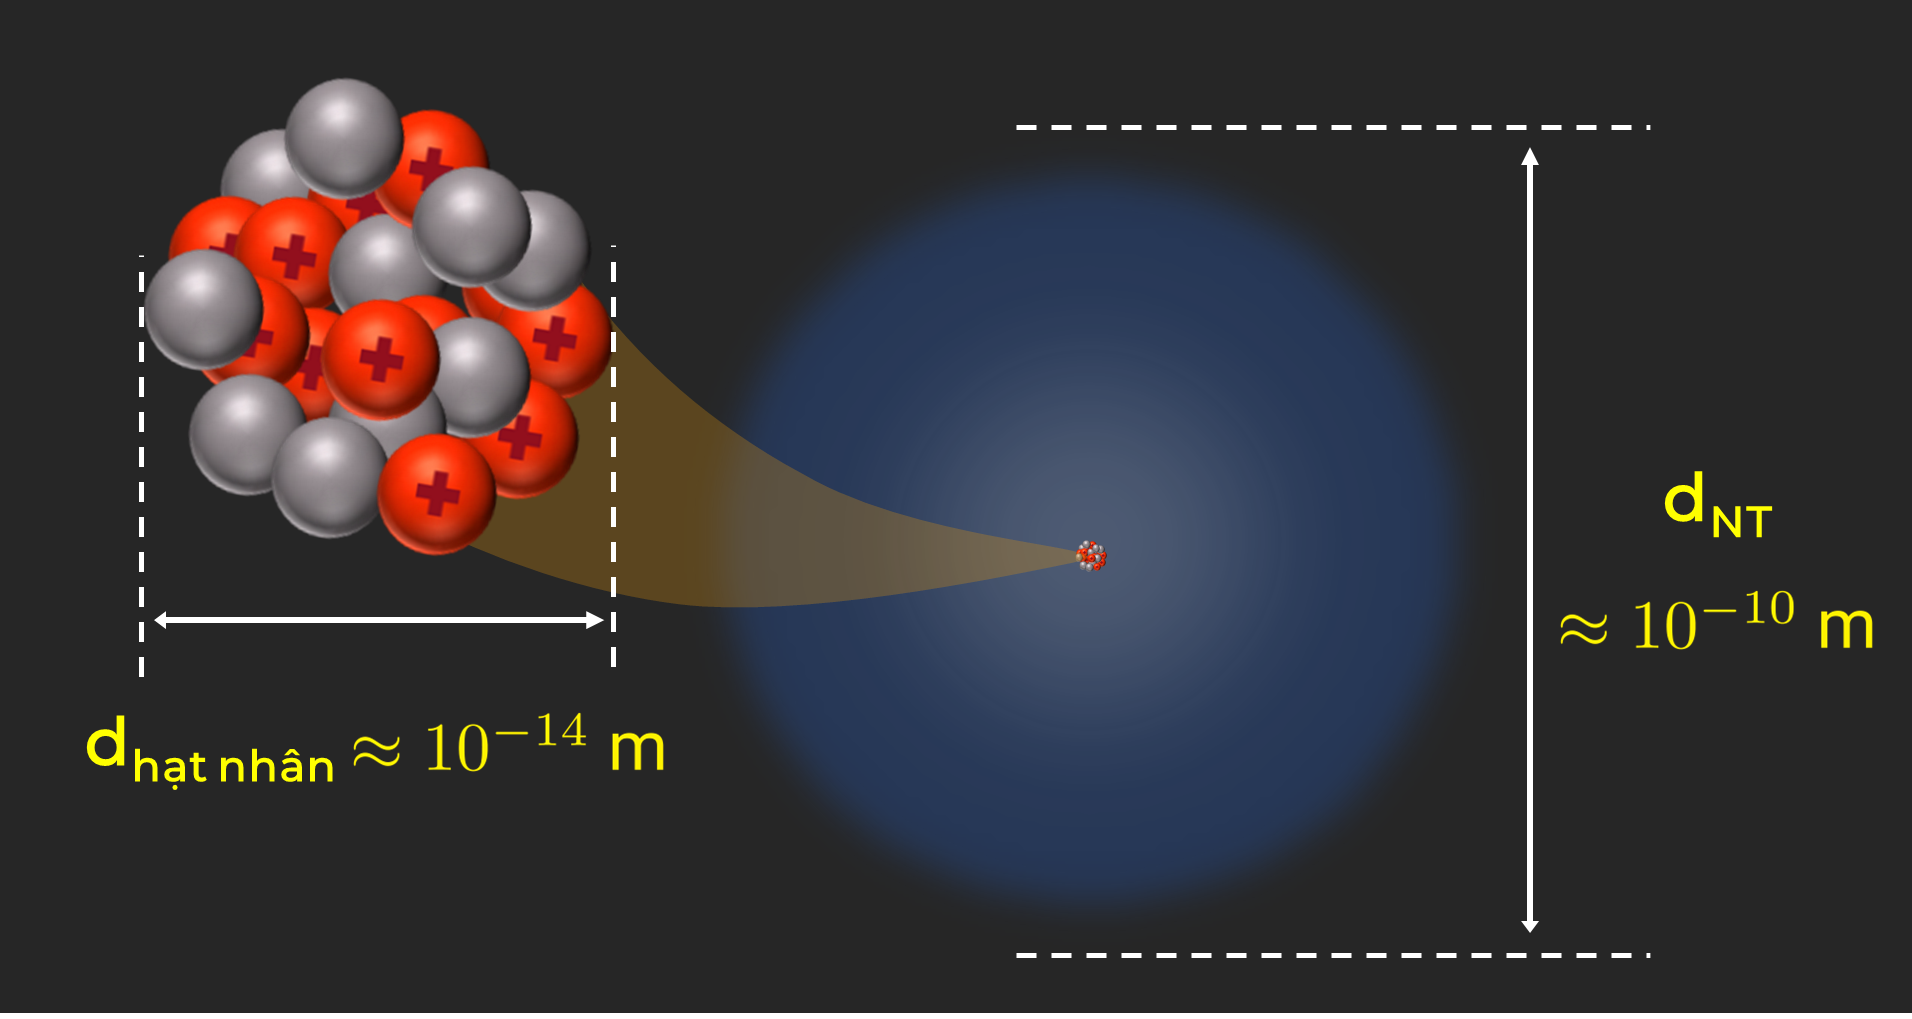
\includegraphics[width=9cm]{ktnt}\\
	\captionof{figure}{So sánh kích thước hạt nhân , nguyên tử}
	\label{fig:hinh7}
\end{center}
\begin{notegsnd}
	\begin{itemize}
		\item Đơn vị kích thước thường dùng của nguyên tử là Angstron ($ A^0 $) hoặc nano mét (nm)			
		$$1 \mathrm{~nm}=10^{-9}~\mathrm{m} ; 1 A^0=10^{-10}~\mathrm{~m} ; 1 \mathrm{~nm}=10 A^0; 1 A^0=10^{2}~\mathrm{pm}$$
		\begin{center}
			\tcbox[width=5cm,colframe=dndo]{$ \dfrac{d_{\text{NT}}}{d_{\text{hạt nhân}}}\approx \dfrac{10^{-10}}{10^{-14}} \approx 10^4~\mathrm{\text{lần}} $}
		\end{center}
		\item Đơn vị của khối lương nguyên tử là amu (atomic mass unit),
		$$
		1 \mathrm{amu}=1,6605 \times 10^{-27} \mathrm{~kg} \text {. }
		$$
		\item Đơn vi của điện tích các hạt cơ bản là $\mathrm{e}_0$ (điện tích nguyên tố),
		$$
		1 \mathrm{e}_0=1,602 \times 10^{-19} \mathrm{C} \text {. }
		$$
	\end{itemize}
\end{notegsnd}
\newpage
\vspace*{3pt}

\ntd{BÀI TẬP TRẮC NGHIỆM}:
\begin{dangntd}{LÝ THUYẾT VỀ CẤU TẠO NGUYÊN TỬ}
	\giaibaitap{Phương pháp giải}
	\begin{itemize}
		\item Nắm vững về cấu tạo nguyên tử
		\item Nắm vững kết quả thí nghiệm của Thomson,Rutherford
	\end{itemize}
\end{dangntd}
\Opensolutionfile{ansbook}[DAPAN/BTTLH10CO102tachLG]
\Opensolutionfile{ans}[DAPAN/BTTLH10CO102]
\begin{ex}[1]
	Các hạt cơ bản của hầu hết các nguyên tử là?
	\choice
	{%
		electron
	}
	{%
		electron và proton
	}
	{%
		proton và notron
	}
	{%
		\True electron, proton và notron
	}
	\sodongkeex[5]
\end{ex}


\begin{ex}[1]
	Hạt nhân của hầu hết các nguyên tử gồm có?
	\choice
	{%
		electron
	}
	{%
		electron và proton
	}
	{%
		\True proton và notron
	}
	{%
		electron, proton và notron
	}
	\sodongkeex[5]
\end{ex}

\begin{ex}[2]
	Trong thí nghiệm của Thomson, phát biểu nào sau đây sai với kết quả thí nghiệm ta quan sát được?
	\choice
	{%
		Tia âm cực là các chùm hạt electron di chuyển từ cực âm sang cực dương
	}
	{%
		Tia âm cực là chùm hạt mang điện tích âm
	}
	{%
		\True	Tia âm cực bị lệch về phía bản cực âm của nguồn điện
	}
	{%
		Tia âm cực bị lệch hướng khi ta đặt nó trong từ trường
	}
	\sodongkeex[5]
\end{ex}

\begin{ex}[2]
	Theo mô hình bánh pudding mận của Thomson, phát biểu nào sau đây là đúng?
	\choice
	{%
		Nguyên tử có cấu tạo rỗng gồm hạt nhân mang điện tích dương và vỏ là các electron chuyển động xung quanh hạt nhân.
	}
	{%
		Nguyên tử có cấu tạo rỗng gồm hạt nhân mang điện tích dương và vỏ là các electron chuyển dộng xung quanh hạt nhân theo những quỹ đạo có kích thước và năng lượng cố định
	}
	{%
		\True	nguyên tử bao gồm các electron nằm rải rác trong một đám mây hình cầu mang điện tích dương.
	}
	{%
		các electron  quay quanh hạt nhân không theo một quỹ đạo xác định, mà chúng tạo thành các đám mây điện tích mà tại đó xác suất tìm thấy electron là lớn nhất
	}
	\sodongkeex[5]
\end{ex}
\begin{ex}[2]
	Cho các phát biểu sau:
	\begin{enumerate}[(1)]
		\item Tất cả các hạt nhân nguyên tử đều được cấu tạo từ các hạt proton và neutron.
		\item Khối lượng nguyên tử tập trung phần lớn ở lớp vỏ.
		\item Trong nguyên tử, số electron bằng số proton.
		\item Trong hạt nhân nguyên tử, hạt mang điện là proton và electron.
		\item Trong nguyên tử, hạt electron có khối lượng không đáng kể so với các hạt còn lại.
	\end{enumerate}
	Số phát biểu đúng là
	\choice
	{%
		1
	}
	{%
		\True 2
	}
	{%
		3
	}
	{%
		4
	}
	\huongdan{%
		Phát biểu đúng là:
		Trong hạt nhân nguyên tử, hạt mang điện là proton và electron.\\
		Trong nguyên tử, hạt electron có khối lượng không đáng kể so với các hạt còn lại
	}
	
\end{ex}

\begin{ex}[2]
	Điều nào sau đây đúng theo mô hình nguyên tử của Thomson?
	\choice
	{%
		Nguyên tử không trung hòa về điện
	}
	{%
		\True Nguyên tử là quả cầu mang điện tích dương có chứa các êlectron bên trong
	}
	{%
		Điện tích âm và điện tích dương trong nguyên tử có độ lớn bằng nhau
	}
	{%
		Không có điều nào ở trên
	}
	\sodongkeex[5]
\end{ex}


\begin{ex}[3]
	Trong hiện tượng xả điện qua khí ở áp suất thấp, sự tỏa sáng màu trong ống xuất hiện là kết quả của:
	\choice
	{% 
		\True va chạm giữa các hạt mang điện được phát ra từ cực âm và nguyên tử của khí
	}
	{% 
		va chạm giữa các electron khác nhau của các nguyên tử trong khí
	}
	{% 
		kích thích các electron trong các nguyên tử
	}	
	{% 
		va chạm giữa các nguyên tử của khí
	}	
	\sodongkeex[5]	
\end{ex}

\begin{ex}[2]
	Mô hình đầu tiên về nguyên tử được đưa ra bởi:
	\choice
	{%
		N. Bohr
	}
	{% 
		E. Goldstein
	}
	{% 
		Rutherford
	}
	{% 	
		\True J.J. Thomson
	}
	\sodongkeex[5]
\end{ex}

\begin{ex}[2]
	Nếu đường kính của nguyên tử khoảng $10^2 \mathrm{pm}$ thì đường kính của hạt nhân khoảng
	\choice
	{%
		$10^2 \mathrm{pm}$
	}
	{%
		$10^{-4} \mathrm{pm}$
	}
	{%
		\True	$10^{-2} \mathrm{pm}$
	}
	{
		$10^4 \mathrm{pm}$
	}
	\sodongkeex[5]
\end{ex}
\Closesolutionfile{ans}
\Closesolutionfile{ansbook}


\newpage
\giaibaitap{BÀI TẬP TỰ LUẬN}
\Opensolutionfile{ansbt}[DAPAN/BT_H10C0102]
\begin{btex}[2]
	Trong thí nghiệm của Rutherford, khi sử dụng các hạt alpha (ion $\mathrm{He}^{2+}$, kí hiệu là $\mathrm{a}$ ) bắn vào lá vàng thì:
	\begin{itemize}
		\item Hầu hết các hạt a xuyên thẳng qua lá vàng.
		\item Một số ít hạt a bị lệch quỹ đạo so với ban đầu.
		\item Một số rất ít hạt a bị bật ngược trở lại.
	\end{itemize}
	Từ kết quả này, em có nhận xét gì về cấu tạo nguyên tử?
	\loigiai{
		Trong thí nghiệm của Rutherford, khi sử dụng các hạt alpha (ion $\mathrm{He}^{2+}$, kí hiệu là a) bắn vào lá vàng thì:
		\begin{itemize}
			\item Hầu hết các hạt a xuyên thẳng qua lá vàng chứng tỏ nguyên tử có cấu tạo rỗng.
			\item Một số ít hạt a bị lệch quỹ đạo so với ban đầu chứng tỏ hạt nhân nguyên tử cùng điện tích dương như hạt hạt alpha (ion $\mathrm{He}^{2+}$, kí hiệu là $ \alpha $).
			\item Một số rất ít hạt a bị bật ngược trở lại chứng tỏ kích thước hạt nhân nhỏ hơn rất nhiều so với kích thước của nguyên tử và khối lượng nguyên tử tập trung chủ yếu ở hạt nhân.
		\end{itemize}
		
	}
\end{btex}

\begin{btex}[2]
	Viết lại bảng sau vào vở và điền thông tin còn thiếu vào các ô trống:\\
	\begin{tabular}{|c|c|c|c|c|c|c|}
		\rowcolor{dnxanh!25} 
		\hline \indam[dnxanhdam]{Nguyên tố} & \indam[dnxanhdam]{Kí hiệu} & \color{dnxanhdam} {$\mathbf{Z}$} & \indam[dnxanhdam]{Số e} & \indam[dnxanhdam]{Số p} & \indam[dnxanhdam]{Số n} & \indam[dnxanhdam]{Số khối} \\
		\rowcolor{dnvang!25} 
		\hline \indam[dnxanhdam]{Carbon} & $\mathrm{C}$ & 6 & 6 & $?$ & 6 & $?$ \\
		\rowcolor{dnvang!25} 
		\hline \indam[dnxanhdam]{Nitrogen} & $\mathrm{N}$ & 7 & $?$ & 7 & $?$ & 14 \\
		\rowcolor{dnvang!25} 
		\hline \indam[dnxanhdam]{Oxygen} & $\mathrm{O}$ & 8 & 8 & $?$ & 8 & $?$ \\
		\rowcolor{dnvang!25} 
		\hline \indam[dnxanhdam]{Sodium (natri)} & $\mathrm{Na}$ & 11 & $?$ & 11 & $?$ & 23 \\
		\rowcolor{dnvang!25}
		\hline \indam[dnxanhdam]{Aluminium (nhôm)} & $\mathrm{Al}$ & $?$ & 13 & $?$ & $?$ & 27 \\
		\hline
	\end{tabular}
	\huongdan{
		\taodongke{5}
	}
\end{btex}

\Closesolutionfile{ansbt}










\newpage
\begin{dangntd}{Bài tập về khối lượng, kích thước nguyên tử}	
	\giaibaitap{Phương pháp giải}\\
	\tieumuc{Các công thức liên quan khối lượng}
	\begin{itemize}
		\item $ m _{\text{nguyên tử}=m_{p}+m_{n} + m_{e} } $ (tính chính xác); $ m _{\text{nguyên tử}} \approx  m_{p} + m_{n} \approx m_{\text{hạt nhân}} $ (tính gần đúng)
		\item Khối lượng tính ra kg của 1 nguyên tử carbon-12 là $ 19,926 . 10^{27}~\mathrm{kg}$.
		\item 1 amu được định nghĩa bằng $\dfrac{1}{12}$ khối lượng 1 nguyên tử carbon-12:
		\item$1 \mathrm{amu}=\dfrac{19,926 \cdot 10^{-27} \mathrm{~kg}}{12}=1,661 \cdot 10^{-27} \mathrm{~kg}$
		\item$1 \mathrm{mol}$ chứa $ 6,02.10^{23} $ nguyên tử, phân tử, ion.
	\end{itemize}
	\tieumuc{Các công thức liên quan kích thước}
	\begin{itemize}
		\item Thể tích của hình cầu:
		$ V=\dfrac{4}{3}\pi r^3 $
		\item Phần trăm thể tích các nguyên tử trong tinh thể $ = \dfrac{V_{\text{các nguyên tử}}}{V_{\text{tinh thể}}}\cdot 100\% $
		\item Một số đơn vị đo: 
		$\left\{\begin{array}{l}
			1~\mathrm{nm} = 10^{-9}~\mathrm{m}\\
			1~\mathrm{A^{0}} = 10^{-10}~\mathrm{m}\\
			1~\mathrm{pm} = 10^{-12}~\mathrm{m}	
		\end{array}\right.$
	\end{itemize}
\end{dangntd}
\begin{vdm}{Ví dụ mẫu}
\end{vdm}

%Câu 1: Khối lượng của nguyên tử magnesium là $39,8271 \cdot 10^{-27} \mathrm{~kg}$. Khối lượng của magnesium theo amu là
%A. 23,978
%B. $66,133 \cdot 10^{-51}$.
%C. 24,000 .
%D. $23,985 \cdot 10^{-3}$.

\begin{vdex}[2]	
	Khối lượng của nguyên tử magnesium là $39,8271 \cdot 10^{-27} \mathrm{~kg}$. Khối lượng của magnesium theo amu là
	\choice
	{%
		\True $ 23,978 $
	}
	{%
		$66,133 \cdot 10^{-51}$
	}
	{%
		$23,985 \cdot 10^{-3}$
	}
	{%
		$ 24,000 $
	}
	\huongdan{
		
	}	
\end{vdex}

\begin{vdex}[2]
	Khối lượng tuyệt đối của một nguyên tử oxygen bằng $26,5595.10^{-27} \mathrm{~kg}$. Hãy tính khối lượng nguyên tử (theo amu) và khối lượng mol nguyên tử (theo g) của nguyên tử này.
	\loigiai
	{%
		$
		1 \mathrm{amu}=1,661 \cdot 10^{-27} \mathrm{~kg}
		$\\
		
		
		Khối lượng của nguyên tử oxygen theo amu là:
		$
		\dfrac{26,5595 \cdot 10^{-27}}{1,661 \cdot 10^{-27}} \approx 15,99~ \mathrm{amu}
		$\\
		
		$1 \mathrm{mol}$ chứa $ 6,02.10^{23} $ nguyên tử\\
		$\Rightarrow$ Khối lượng mol của oxygen là  $=26,5595.10^{-24}.6,02.10^{23}= 15,99~ \mathrm{gam} $
		
	}
\end{vdex}

%Câu 3: Nguyên tử helium có 2 proton, 2 neutron và 2 electron. Khối lượng của các electron chiếm baoo nhiêu $\%$ khối lượng nguyên tử helium?
%A. $2,72 \%$.
%B. $0,272 \%$.
%C. $0,0272 \%$.
%D. $0,0227 \%$.

\begin{vdex}[2]
	Nguyên tử helium có 2 proton, 2 neutron và 2 electron. Khối lượng của các electron chiếm bao nhiêu $\%$ khối lượng nguyên tử helium?
	\choice
	{%
		$2,72 \%$
	}
	{%
		$0,272 \%$
	}
	{%
		\True	$0,0272 \%$
	}
	{%
		$0,0227 \%$
	}
	\huongdan
	{%
		Khối lượng nguyên tử helium là:\\ $ m_{NT} = 2m_{p} + 2m_{n} + 2m_{e} = 2.1,672.10^{-27} + 2.1,675.10^{-27} + 2 .9,109.10^{-31} = 6.696.10^{-27}~\mathrm (kg) $\\
		Phần trăm khối lượng của electron trong nguyên tử helium là:\\
		$ \%m_{e}=\dfrac{2 .9,109.10^{-31}}{5.51941.10^{-27}}.100\%=0,0272 \%$
		
	}
\end{vdex}



\begin{vdex}[2]
	Khối lượng riêng của canxi kim loại  là $ 1,55 g/cm^3 $. Giả thiết rằng , trong tinh thể canxi các nguyên tử là những hình cầu chiếm $ 74\% $ thể tích tinh thể, phần còn lại là khe rỗng.Bán kính nguyên tử tính theo lý thuyết là
	\choice
	{%
		$0,185~\mathrm{nm}$
	}
	{%
		\True	$0,196~\mathrm{nm}$
	}
	{%
		$0,155~\mathrm{nm}$
	}
	{%
		$0,168~\mathrm{nm}$
	}
	\huongdan
	{%
		Lấy 1 mol Ca\\
		Ta có: $ D_{Ca}=\dfrac{m_{Ca}}{V_{\scriptsize\text{tinh thể Ca}}}=\dfrac{M_{Ca}.1}{V_{\scriptsize\text{tinh thể Ca}}}\Rightarrow V_{\scriptsize\text{tinh thể Ca}} = \dfrac{M_{Ca}}{D_{Ca}} ~\mathrm{cm^{3}} $\\
		Thể tích 1 mol ca là: $ V_{\scriptsize\text{ 1 mol Ca} } = \dfrac{74}{100} \cdot V_{\scriptsize\text{tinh thể Ca}} = \dfrac{74}{100} \cdot \dfrac{M_{Ca}}{D_{Ca}} $\\
		Thể tích một nguyên tử Canxi là:
		$V_{\scriptsize\text{1 NT Ca}} = \dfrac{V_{\scriptsize\text{ 1 mol Ca}}}{6,02.10^{23}}=\dfrac{74.M_{Ca}}{6,02.10^{23}.100.D_{Ca}} $\\
		$ \Rightarrow \dfrac{4}{3}\pi r^{3} = \dfrac{74.M_{Ca}}{6,02.10^{23}.100.D_{Ca}} \Rightarrow \dfrac{4}{3}\pi r^{3} = \dfrac{74.40}{6,02.10^{23}.100.1,55} \Rightarrow r= 1,96.10^{-8}~\mathrm{cm}=0,196 ~\mathrm{nm} $ 
	}
\end{vdex}

\begin{bttl}{Bài tập tự luyện}
\end{bttl}
\ntd{Bài tập trắc nghiệm}
\Opensolutionfile{ans}[DAPAN/BTTLH10C010202]
\setcounter{tcb@cnt@exbox}{0}
\begin{ex}[2]
	Bán kính nguyên tử và khối lượng mol của nguyên tử $ Fe $ lần lượt là $ 1,28 A^{0} $ và $ 56  $ gam/mol . Biết rằng trong tinh thể $ Fe $ chỉ chiếm $ 74\% $ về thể tích, còn lại là rỗng. Khối lượng riêng của sắt là
	\choice
	{%
		\True	$ 7,84 ~\mathrm{gam /cm^{3}}$
	}
	{%
		$ 8,74 ~\mathrm{gam /cm^{3}}$
	}
	{%
		$ 4,78 ~\mathrm{gam /cm^{3}}$
	}
	{%
		$ 7,48 ~\mathrm{gam /cm^{3}}$
	}
\end{ex}


\begin{ex}[3]
	Bán kính nguyên tử và khối lượng mol của nguyên tử $ Fe $ lần lượt là $ 1,28 A^{0} $ và $ 56  $ gam/mol . Biết rằng trong tinh thể $ Fe $ chỉ chiếm $ 74\% $ về thể tích, còn lại là rỗng. Khối lượng riêng của sắt là
	\choice
	{%
		\True	$ 7,84 ~\mathrm{gam /cm^{3}}$
	}
	{%
		$ 8,74 ~\mathrm{gam /cm^{3}}$
	}
	{%
		$ 4,78 ~\mathrm{gam /cm^{3}}$
	}
	{%
		$ 7,48 ~\mathrm{gam /cm^{3}}$
	}
\end{ex}

\Closesolutionfile{ans}

\ntd{Bài tập tự luận}
\Opensolutionfile{ansbt}[DAPAN/BTTL_H10C010202_TL]

\begin{btex}[2]
	Nguyên tử aluminium (nhôm) gồm 13 proton và 14 neutron. Tính khối lượng proton, neutron, electron có trong $27 \mathrm{~g}$ nhôm.
	\loigiai{
		Ta có : $ n_{Al}=\dfrac{m_{Al}}{M_{Al}}= \dfrac{27}{27}=1~\mathrm{mol}\\ $	
		$ \Rightarrow $ Khối lượng proton là: $ 13.1,672.10^{-24}.6,02.10^{23} =13,0972 ~\mathrm{gam} $\\
		Khối lượng neutron là: $14 \cdot 1,675 \cdot 10^{-24} \cdot 6,022 \cdot 10^{23}=14,1216(\mathrm{~g})$.\\
		Khối lượng electron là: $13 \cdot 9,109 \cdot 10^{-28} \cdot 6,022 \cdot 10^{23}=7,131 \cdot 10^{-3}(\mathrm{~g})$.\
	}
\end{btex}

\begin{btex}[3]
	Nguyên tử $\mathrm{Fe}$ ở $20^{\circ} \mathrm{C}$ có khối lượng riêng là $7,87 \mathrm{~g} / \mathrm{cm}^3$. Với giả thiết này, tinh thể nguyên tử Fe là những hình cầu chiếm $75 \%$ thể tích tinh thể, phần còn lại là những khe rỗng giữa các quả cầu. Cho biết khối lượng nguyên tử của Fe là 55,847 . Tính bán kính nguyên tử gần đúng của $\mathrm{Fe}$.
	\loigiai
	{%
		\noindent Lấy 1 mol Fe
		Ta có: $ D_{Fe}=\dfrac{m_{Fe}}{V_{\scriptsize\text{tinh thể Fe}}}=\dfrac{M_{Fe}.1}{V_{\scriptsize\text{tinh thể Fe}}}\Rightarrow V_{\scriptsize\text{tinh thể Fe}} = \dfrac{M_{Fe}}{D_{Fe}} ~\mathrm{cm^{3}} $\\
		Thể tích 1 mol Fe là: $ V_{\scriptsize\text{ 1 mol Fe} } = \dfrac{75}{100} \cdot V_{\scriptsize\text{tinh thể Fe}} = \dfrac{75}{100} \cdot \dfrac{M_{Fe}}{D_{Fe}} $\\
		Thể tích một nguyên tử Fe là:
		$V_{\scriptsize\text{1 NT Ca}} = \dfrac{V_{\scriptsize\text{ 1 mol Fe}}}{6,02.10^{23}}=\dfrac{75.M_{Fe}}{6,02.10^{23}.100.D_{Fe}} $\\
		$ \Rightarrow \dfrac{4}{3}\pi r^{3} = \dfrac{75.M_{Fe}}{6,02.10^{23}.100.D_{Fe}} \Rightarrow \dfrac{4}{3}\pi r^{3} = \dfrac{75.55,847}{6,02.10^{23}.100.7,87} \Rightarrow r= 1,28.10^{-8}~\mathrm{cm}=0,128 ~\mathrm{nm} $ 
	}
\end{btex}

\begin{btex}[3]
	Nguyên tử kẽm $(\mathrm{Zn})$ có nguyên tử khối bằng 65 . Thực tế hầu như toàn bộ khối lượng nguyên tử tập trung ở hạt nhân, với bán kinh $r=2 \times 10^{-15} \mathrm{~m}$. Khối lượng riêng của hạt nhân nguyên tử kẽm là bao nhiêu tấn trên một centimet khối (tấn/cm³)?
	\loigiai{
		\noindent Đổi $\mathrm{r}=2 \times 10^{-15} \mathrm{~m}=2 \times 10^{-13} \mathrm{~cm}$.\\
		Thể tích hạt nhân nguyên tử Zn:$ =\dfrac{4}{3}\pi r^{3} =\dfrac{4}{3}\pi (2x10^{-13})^{3}=3,349.10^{-38}~\mathrm{cm^{3}} $\\
		Ta có $1 \mathrm{u}=1,66.10^{-27} \mathrm{~kg}=1,66.10^{-30}$ tấn.\\
		Khối lượng riêng của hạt nhân nguyên tử Zn là:
		$
		d=\dfrac{65.1,66 \cdot 10^{-30}}{3,349 \cdot 10^{-38}}=3,22.10^9\left(\text { tấn } / \mathrm{cm}^3\right. \text { ) }
		$
	}
\end{btex}


\Closesolutionfile{ansbt}

\newpage
\begin{dangntd}{Bài tập về các loại hạt}
	\giaibaitap{Phương pháp giải}\\
	\tieumuc{Các loại hạt của nguyên tử}\\
	\begin{itemize}
		\item	Xét nguyyên tử X. Gọi Z là số proton của Z
		$ \Rightarrow $ Số electron của X là Z.
		Gọi N  là số nơtron của X.
		\begin{itemize}
			\item Số hạt mang điện của nguyên tử X là \indam[dndo]{$ \mathbf= $ số p $\mathbf + $ số e $\mathbf = 2Z +N $}
			\item Số hạt mang điện dương của nguyên tử X là \indam[dndo]{$\mathbf = $ số p $ \mathbf = Z  $}
			\item Số hạt mang điện âm của nguyên tử X là \indam[dndo]{ {$ \mathbf = $} số e $\mathbf = $ số p $\mathbf  = Z  $}
		\end{itemize}
		\item Đối với các nguyên tố có số proton từ 2 đến 82 $ (2<Z<82) $.Ta luôn có : \indam[dndo]{$\mathbf{1<\dfrac{N}{Z} <1,5} $}
		\item Xét hợp chất $ M $ có công thức là $ X_{n}Y_{m} $
		\begin{itemize}
			\item Số proton của $ M $ là $ n.Z_{X} + m.Z_{Y} $
			\item Số electron của $ M $ là $ n.Z_{X} + m.Z_{Y} $
			\item Số nơtron của $ M $ là $ n.N_{X} + m.N_{Y} $
		\end{itemize}
	\end{itemize}
	\tieumuc{Các loại hạt của ion}\\
	\begin{itemize}
		\item Nguyên tử trung hòa về điện khi  mất bớt electron trở thành ion dương (cation)
		\begin{center}
			\tcbox[colback=dndo!15,frame hidden,colframe=dndo]{$X  \longrightarrow X^{n+} + ne $}
		\end{center}
		\begin{itemize}
			\item Số proton của $ X^{n+} = Z $.
			\item Số electron của $ X^{n+} = Z-n $.
			\item Số nơtron của $ X^{n+} = N $.
		\end{itemize}
		
		\item Nguyên tử trung hòa về điện khi nhận thêm electron trở thành ion âm (anion)
		\begin{center}
			\tcbox[colback=dndo!15,frame hidden,colframe=dndo]{$ X + me \longrightarrow X^{m+} $}
		\end{center}
		\begin{itemize}
			\item Số proton của $ X^{m-} = Z $.
			\item Số electron của $ X^{m-} = Z+m $.
			\item Số nơtron của $ X^{m-} = N $.
		\end{itemize}
	\end{itemize}
\end{dangntd}
\begin{vdm}{Ví dụ mẫu}
\end{vdm}

\begin{vdex}[2]
	Nguyên tử nguyên tố X có tổng số hạt cơ bản là 40. Trong đó số hạt mang điện nhiều hơn số hạt không mang điện là 12. Nguyên tố X là:
	\choice
	{%
		\True	Al
	}
	{%
		Na
	}
	{%
		Ca
	}
	{%
		F
	}
	\huongdan{
		Gọi Z là số proton và N là số nơtron có trong nguyên tử X.\\
		Theo đề bài nguyên tử X có tổng số hạt cơ bản là $ 40 $ nên ta có:
		$ P + E + N = 40  $\\
		Vì P=E nên:
		\begin{equation}
			\Rightarrow 2Z + N = 40 \label{eq:1}
		\end{equation} 
		
		Mặt khác số hạt mang điện  nhiều hơn số hạt không mang điện là 12, nên ta có: 
		\begin{equation}
			2Z-N=12 \label{eq:2}
		\end{equation}
		
		Từ \eqref{eq:1} và \eqref{eq:2} ta có hệ phương trình:
		$ \begin{cases}
			2Z+N=40\\
			2Z-N =12
		\end{cases} $
		$ \Rightarrow  
		\begin{cases}
			Z=13\\
			N =14
		\end{cases} $ 
		Vậy X là nguyên tố Al (nhôm)
	}
	
\end{vdex}

\begin{vdex}[2]
	Tổng số hạt proton,nơtron, electron trong nguyên tử của nguyên tố X là 46. Biết rằng công thức oxit của X có dạng $ X_{2}O_{5} $.X là nguyên tố
	\choice
	{%
		N
	}
	{%
		\True	P
	}
	{%
		O
	}
	{%
		S
	}
	\huongdan{
	}
\end{vdex}


\begin{vdex}[2]
	Tổng số hạt proton,nơtron, electron trong nguyên tử của nguyên tố X là 46. Biết rằng công thức oxit của X có dạng $ X_{2}O_{5} $.X là nguyên tố
	\choice
	{%
		N
	}
	{%
		\True	P
	}
	{%
		O
	}
	{%
		S
	}
	\huongdan{
	}
\end{vdex}

\begin{bttl}{Bài tập tự luyện}
\end{bttl}
\Opensolutionfile{ans}[DAPAN/BTTL_H10C010203]
\setcounter{tcb@cnt@exbox}{0}
\begin{ex}[2]
	Nguyên tử của một nguyên tố X có tổng số hạt cơ  bản là 82.Biết Số hạt mang điện nhiều hơn số hạt không mang điện là 22. Tổng số proton và nơtron của X là :
	\choice
	{%
		58
	}
	{%
		57
	}
	{%
		\True	56
	}
	{%
		55
	}
	
\end{ex}


\begin{ex}[2]
	Tổng số hạt trong cation $ R^{2+} $ là 58. Trong nguyên tử R số hạt mang điện nhiều hơn số hạt không mang điện là 20 hạt. Số electron của cation $ R^{2+} $ là
	\choice
	{%
		\True	18
	}
	{%
		22
	}
	{%
		20
	}
	{%
		16
	}
\end{ex}

\begin{ex}[2]
	Nguyên tử của nguyên tố Y có tổng số hạt là 16. Số electron của nguyên tử Y là
	\choice
	{%
		7
	}
	{%
		6
	}
	{%
		\True	5
	}
	{%
		8
	}
\end{ex}

\begin{ex}[3]
	Tổng số electron trong ion $ AB_{3}^{-} $ là $ 32 $ hạt. Số hạt mang điện trong nguyên tử A nhiều hơn số hạt trong hạt nhân nguyên tử B là 6 hạt. Số proton của A và B lần lượt là:
	\choice
	{%
		6 và 7
	}
	{%
		\True	7 và 8
	}
	{%
		8 và 9
	}
	{%
		5 và 6
	}
\end{ex}

\begin{bt}[2][Bài tập 1.11 SBT hóa 10 KNTT]
	Hợp kim chứa nguyên tố $\mathrm{X}$ nhẹ và bền, dùng chế tạo vỏ máy bay, tên lửa. Nguyên tố $\mathrm{X}$ còn được sử dụng trong xây dựng, ngành điện và đồ gia dụng. Nguyên tử của nguyên tố $\mathrm{X}$ có tổng số hạt (proton, electron, neutron) là 40 . Tổng số hạt mang điện nhiều hơn tổng số hạt không mang điện là 12 .
	\begin{enumerate}[a)]
		\item Tính số mỗi loại hạt (proton, electron, neutron) trong nguyên tử $\mathrm{X}$.
		\item Tính số khối của nguyên tử $\mathrm{X}$.
	\end{enumerate}
%\sodongkebt[5]
\huongdan{
\taodongke{5}
}
\end{bt}
\Closesolutionfile{ans}